\section{Flujo de trabajo completo}
Todas las tareas que hemos ido indicado durante este documento se deben
incorporar al grafo que representa el flujo de trabajo que se ejecuta en
Airflow. El grafo final que he implementado se puede ver en la figura
\ref{fig:workflow}.

\begin{itemize}
    \item\href{
        https://github.com/Varrrro/forecast/blob/master/airflow/tasks.py#L210-L224
    }{Definición de las dependencias entre tareas}
\end{itemize}

\begin{figure}[h!]
    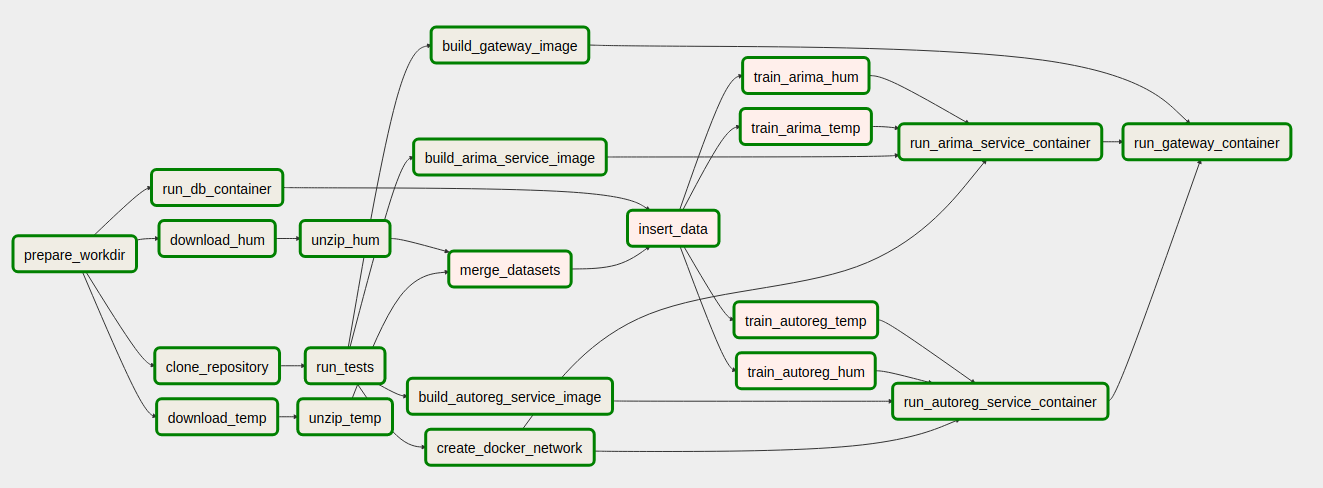
\includegraphics[width=\textwidth]{images/workflow.png}
    \caption{Grafo del flujo de trabajo.}
    \label{fig:workflow}
\end{figure}
